% Chapter 20 -- English translation of chapters/c20.tex (French source): RK4 cools at resolved steps, it does not heat (edition 2, refuting the premise of edition 1)
% Figure: code/fig20.py.
\chapter[The thermostat on trial]{The thermostat was accused of overheating}
\reference{Edition~1 deposited on 19 October 2026 in seven copies (including \doi{10.5281/zenodo.23478809}). Edition~2, which refutes it, published on 21 October 2026: \doi{10.5281/zenodo.23532458}.}

\noindent\niveau{X} for the numerical experiment; \niveau{As} for the Lean statements on the linear case (axiom
audit passed, without a complete replay in the kernel).

\section*{The idea in one picture}

\begin{analogie}
A family accuses the thermostat of slowly overheating the house. Someone finally puts thermometers in every room,
for weeks: the thermostat does not overheat, it keeps the house a little too \emph{cold}; at large steps, it really
does start to heat.

\emph{Where the picture stops:} here, ``heating'' and ``cooling'' denote an error in the calculated energy of a
particle, not a temperature; and with calculation steps that are too large, the method really does start to heat.
\end{analogie}

\section*{What was done}

On 19 October, a batch of papers appeared under the label ``peer reviewed in five rounds''. One of them, deposited
seven times, was about the confinement of particles in a stellarator, a fusion machine that traps a plasma in a
magnetic field. It justified a calculation method by a claim: the classical method, called RK4, would slowly
``heat'' the trapped particles through numerical error, until they crossed the magnetic barrier and escaped.

Two days later, edition~2 \emph{measured} that claim in the very model that edition~1 was computing: a simplified
magnetic well with two degrees of freedom, whose escape energy is known exactly, $H^*=29/40$. The protocol:
2\,000 randomly drawn orbits per energy band, five time steps from $0.05$ to $0.8$, a duration of 2\,000, and a
verdict rule written before the calculations. Result: below the threshold, at every time step, 100~\% of the RK4
orbits end with \emph{less} energy than they started with, without a single spurious escape. The hypothesis is
refuted. The real weakness of RK4 is the opposite: above the threshold, a very accurate reference calculation lets
$61.8$~\% of the orbits escape; RK4 lets as many escape at small steps, but only $46.4$~\% at step $0.4$ and
$9.05$~\% at step $0.8$ (figure~\ref{fig:c20}). It holds back particles that should leave.

\paragraph{An example to follow with a pencil.} Take the simplest case, a perfect spring: position $x=1$,
velocity $p=0$, energy proportional to $x^2+p^2=1$, and a calculation step such that $y=\omega h=1$. Euler's method gives
$x=1$, $p=-1$: energy $2$, it has doubled. RK4 multiplies the energy by
\[
1-\frac{1}{72}+\frac{1}{576}=\frac{576-8+1}{576}=\frac{569}{576}\approx0.988,
\]
a little less than~1: it cools. In Lean, the general formula $1-y^6/72+y^8/576$ is proved, as well as the fact that
it stays below~1 as long as $y^2<8$. Beyond that, it exceeds~1: RK4 heats and becomes unstable, hence the
``at resolved steps'' of the title.

\section*{How we made sure it is not wrong}

The experiment had six controls, all of which had to pass before anyone looked at RK4, and they passed. The most
telling is the one that \emph{must fail}: Euler's method and the midpoint method, which provably heat, do produce
spurious escapes; Euler makes all 2\,000 orbits below the threshold escape, at every step. The test was therefore
capable of seeing heating had there been any. The RK4 gaps are judged on the same orbits as the reference:
indistinguishable at the two smallest steps, overwhelming at the two largest. The 18 Lean statements pass the
bench's axiom audit (only the three standard axioms), but without a complete replay in the kernel. For this book,
the fractions in the figure were recomputed from the counts in the published results file.

Edition~2 also withdraws what had no foundation: a ``calibrated confidence'' of $0.9150$, which was a constant
written in the code; a ``multi-round review'' that called no reviewer; figures drawn from formulas and not from
calculations; a theorem attributed to a book that dealt with a different equation.

\section*{What this does not say}

\begin{limite}
\begin{itemize}
\item This is a toy model with two degrees of freedom, not a real stellarator. Nothing is said about real fusion
  codes.
\item The result holds at resolved steps; at large steps, RK4 really does heat.
\item The verdict rule was written before the calculations, but the script was not yet recorded in the
  repository's history: the order of events rests on the author's notes and the file dates.
\item The ``relaxation'' method lets too many orbits escape at the largest step ($68.75$~\%); the paper measures
  this effect but has no explanation for it.
\item The paper itself says that nobody other than the author has reviewed it.
\end{itemize}
\end{limite}

\section*{Going further}

Edition~2, its script, its raw results and its Lean files are at \doi{10.5281/zenodo.23532458}. On the same
21 October, four other withdrawals corrected the batch of the 19th: a method written down in black and white is not
enough, it has to be run.

\begin{figure}[t]
\centering
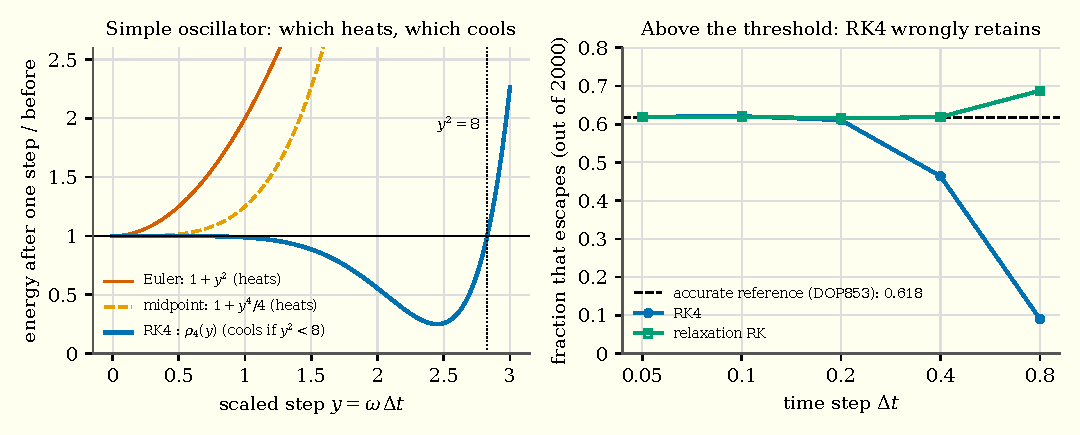
\includegraphics[width=\linewidth]{figures/c20_rk4}
\caption{Left: energy after one step on a perfect spring, computed here and equal to the proved formulas; RK4 cools
as long as $y^2<8$. Right: fraction of the orbits above the threshold that escape, from the published counts: RK4
holds back too many at large steps.}
\label{fig:c20}
\end{figure}
